\msusection{Program Control Window}\label{sec:programcontrol}
Upon executing YCweather.exe, the window that appears is the Program Control window, see Figure~\ref{fig:programcontrol}.  This window acts as the central controls for all operations performed by YCweather. This section focuses on the main purpose of YCweather: creating graphs of weather data.  The Program Control window contains four basic parts: 
\begin{enumerate}
	\item the menus, which are drop-down items at the top of the window (e.g., File menu and Plot menu); 
	\item the toolbar, which contains the buttons just below the menus that act as shortcuts to common menu items;
	\item the Date/Time panel, which contains the options for selecting the date range of interest; and
	\item the Station panel, which lists the weather stations in the database.
\end{enumerate}

\begin{figure}[ht!]\centering
	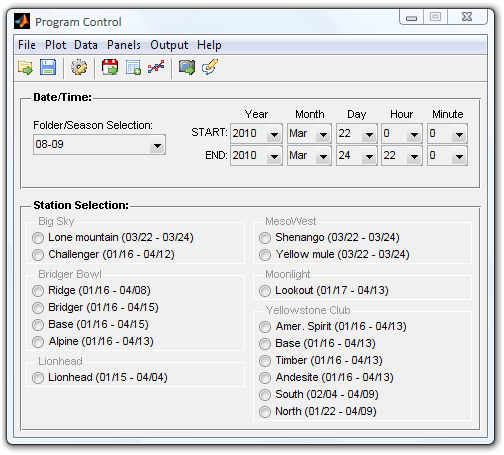
\includegraphics[width=4in]{\YCfiles figures/programcontrol.png}
	\caption{YCweather Program Control window.}\label{fig:programcontrol}
\end{figure}

\msusection{Tutorial: Plotting Weather Data}\label{sec:tutorial}
To quickly create a simple plot of weather data:
\begin{enumerate}
	\item Select a folder from the Folder/Season drop-down option on the Date/Time panel.
	\item Select a weather station from the buttons in the Station panel, for example Ridge and Bridger from Bridger Bowl.
	\item Choose a start and end date from the drop-down menus, be sure to select a range that lies within the available data, which is given in the parenthesis adjacent to the station radio buttons.	
	\item Select the Open Data List option.  This is available by selecting Open Data List option from the Data menu, pressing the Open Data List button on the toolbar, or by pressing CTRL + V.  This will open an additional window, as shown in Figure \ref{fig:datalist}. 
Note, this window may take several seconds to open especially if multiple stations are selected and/or if the stations contain a lot of data.  The reason being that when this window is open the program is recalling all of the data for each station and storing it in a temporary location. This allows the plots to be generated quickly.
	\item In this new window (named Data List) select a weather parameter, such as Air Temperature.  Notice, that when you press a button that all variables without the panel labeled Temperature disappear.  This will prevent plotting of variables with different units on the same axis.	
	\item Finally, plot the data.  This can be done by pressing the Plot Weather Data toolbar button on either Program Control or Data List window, by selecting Weather Data from the Plot menu on either window, and by CTRL + W.
\end{enumerate}

\begin{figure}[ht!]\centering
	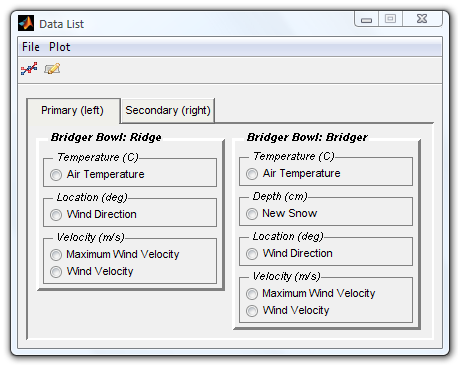
\includegraphics[width=4in]{\YCfiles figures/datalist.png}
	\caption{Example of the Data List window.}\label{fig:datalist}
\end{figure}
































